\documentclass[english]{beamer} %,handout
\usepackage{amsmath}
\usepackage{graphicx}
\usepackage[cjk,hangul,usecjkt1font]{kotex}

\makeatletter

\usepackage{listings}

\setbeamercovered{transparent}

\usecolortheme{kesl}

\usepackage[absolute,overlay]{textpos}
\setlength{\TPHorizModule}{\paperwidth}
\setlength{\TPVertModule}{\paperheight}
\textblockorigin{0mm}{0mm}
 
\usepackage{babel}
\beamertemplatenavigationsymbolsempty
\usepackage{verbatim}
\begin{document}

\title[Memory Scalability]{
A Lightweight Log-based Deferred Update for Linux Kernel
Scalability}

\author{Joohyun Kyong and Sung-Soo Lim}
\institute[Kookmin University]
{
  School of Computer Science\\
  Kookmin University
}

\setbeamercovered{dynamic} 
%TODO Audit Words, reduce

\begin{frame}
  \titlepage
\end{frame}

\begin{frame}{Outline}
	\begin{itemize}
	\item Background of research 
	\item Our new method and Evaluation
	\item Future plans and Summary
	\end{itemize}
\end{frame}

\begin{frame}{AIM7 Scalability - Linux 4.5.0}
\pgfdeclareimage[width=\paperwidth]{background_1}{.//slides/background_1}
\begin{textblock}{1}(0,0)
\pgfuseimage<+->{background_1}
\end{textblock}
\end{frame}

\begin{frame}{Operating System Scalability}
\pgfdeclareimage[width=\paperwidth]{background_2}{.//slides/background_2}
\begin{textblock}{1}(0,0)
\pgfuseimage<+->{background_2}
\end{textblock}
\end{frame}

\begin{frame}{An Analysis of Linux Scalability to Many Cores - OSDI'10}
    \begin{itemize}
    \item Author : Silas Boyd-Wickizer, Austin T.Clements : MIT PDOS
    \item Problem : Linux Scalability 
        \begin{itemize}
        \item Linux Scalability의 문제 분석
        \end{itemize}
    \item Solution : 벤치마크 구현 + 문제 해결
        \begin{itemize}
        \item MOSBench 구현
        \item Per-core data structure 
        \item Eliminating false sharing
        \item Avoiding unneccessary locking
        \item Sloppy counters
        \item Multicore packet processing
        \end{itemize}
    \end{itemize}
\end{frame}

\begin{frame}{An Analysis of Linux Scalability to Many Cores - OSDI'10 }
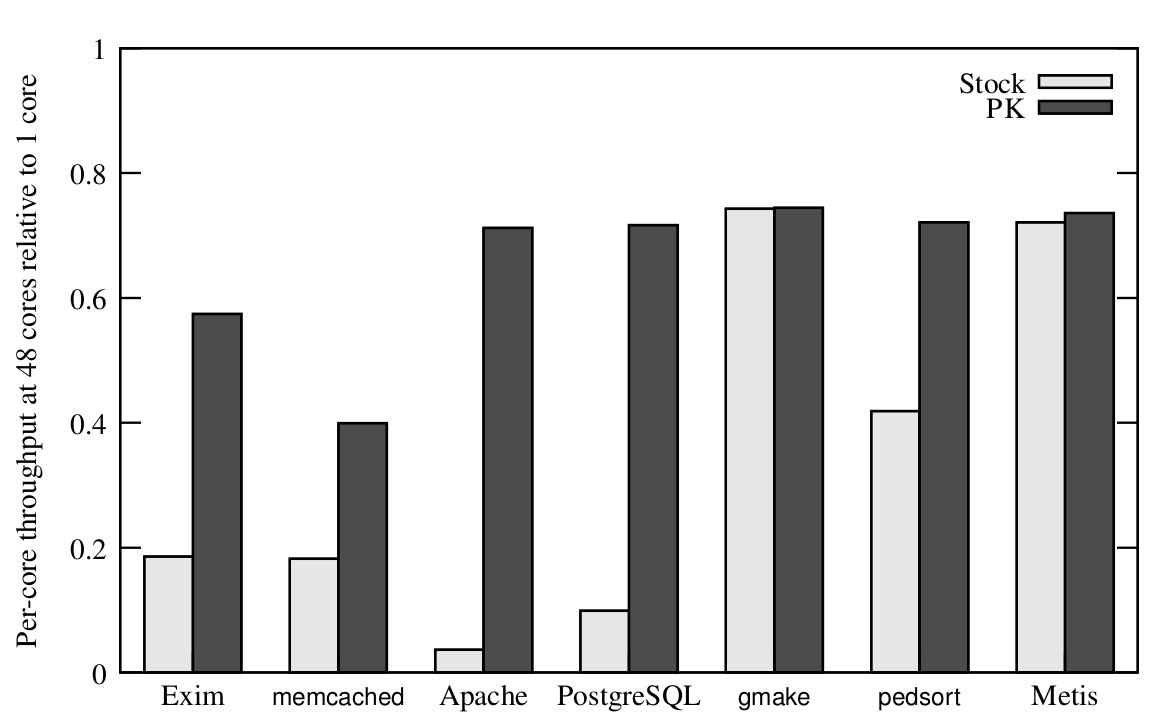
\includegraphics[width=\textwidth,height=0.6\textheight,
keepaspectratio]{scalability}
\end{frame}

\begin{frame}{Non-scalable locks are dangerous - OLS 2012 }
    \begin{itemize}
    \item Author :  Silas Boyd-Wickizer - MIT PODS
    \item Problem : Non-scalable locks 
        \begin{itemize}
        \item 리눅스가 Non-scalable locks 사용
        \end{itemize}
    \item Solution : MCS lock을 사용하자
        \begin{itemize}
        \item MCS lock을 리눅스에 구현 후 실험
        \item 성능 향상
        \end{itemize}
    \end{itemize}
\end{frame}

\begin{frame}{Non-scalable locks are dangerous - OLS 2012 }
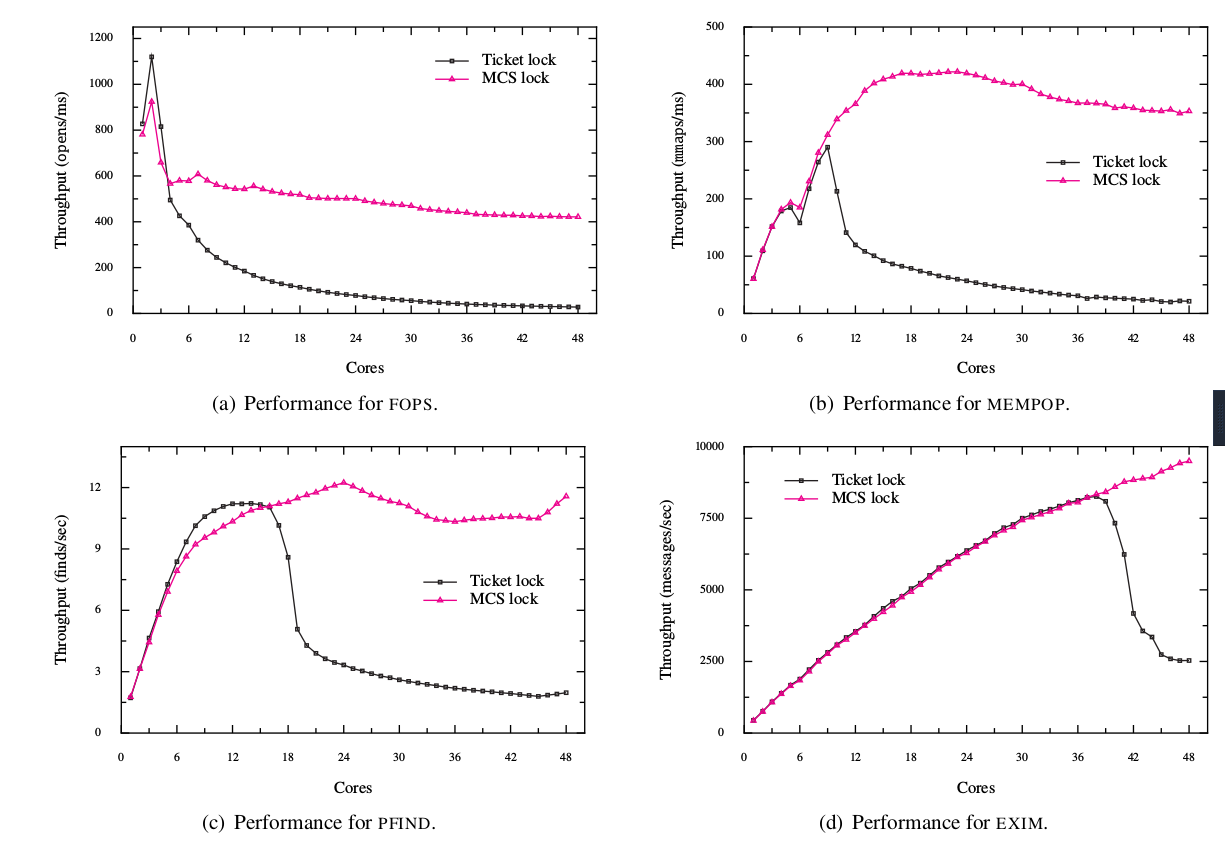
\includegraphics[width=\textwidth,height=0.8\textheight,
keepaspectratio]{mcs}
\end{frame}


\begin{frame}{Scalable Address Spaces Using RCU Balanced Trees - ASPLOS’12} 
    \begin{itemize}
    \item Author : Austin T.Clements : MIT PDOS
    \item Problem : Contention Problem
        \begin{itemize}
        \item mmap + munmap + page faults 
        \end{itemize}
    \item Solution : RCU 이용(BONSAI)
        \begin{itemize}
        \item Linux Red-black tree
        \item RCU balanced tree 
        \end{itemize}
    \end{itemize}
    %\vspace{-2.5cm} 
    %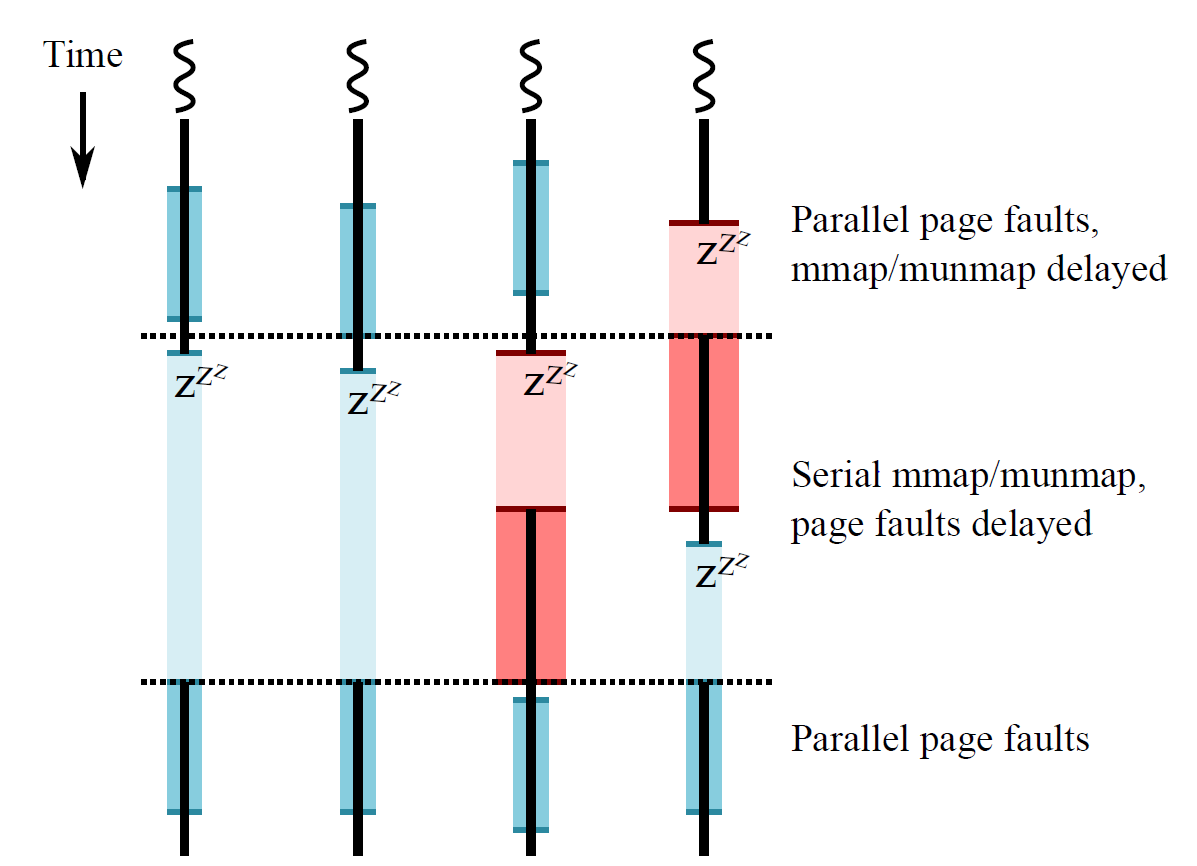
\includegraphics[width=0.4\textwidth,right]{bonsai1}
\end{frame}

\begin{frame}{Scalable Address Spaces Using RCU Balanced Trees - ASPLOS’12} 
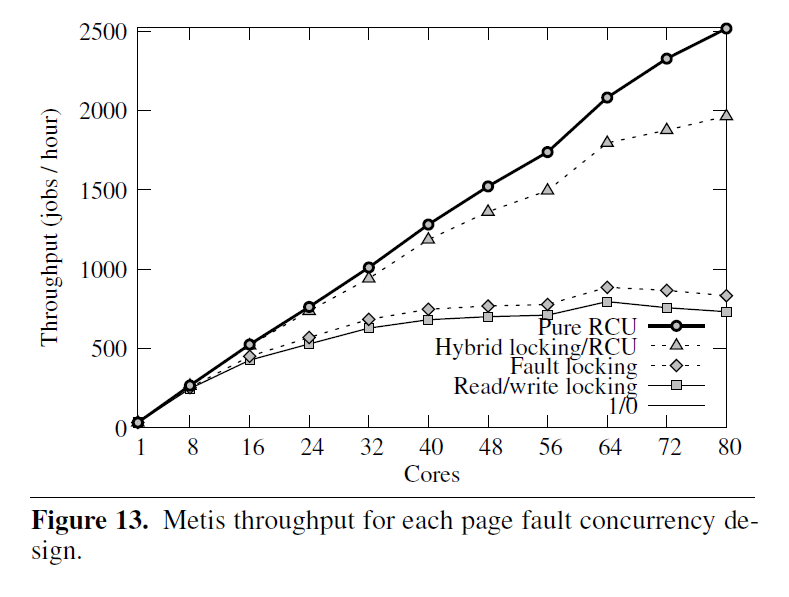
\includegraphics[width=\textwidth,height=0.8\textheight,
keepaspectratio]{bonsai2}
\end{frame}

\begin{frame}{RadixVM: Scalable address spaces for multithreaded applications -
EuroSYS’13}
    \begin{itemize}
    \item Author : Austin T.Clements : MIT PDOS
    \item Problem : Contention Problem
        \begin{itemize}
        \item mmap + munmap + page faults 
        \end{itemize}
    \item Solution : Lockless VM
        \begin{itemize}
        \item TLB shutdown interrupt
        \item Scalable reference counters
        \end{itemize}
    \end{itemize}
    %\vspace{-2.5cm} 
    %\only<1>{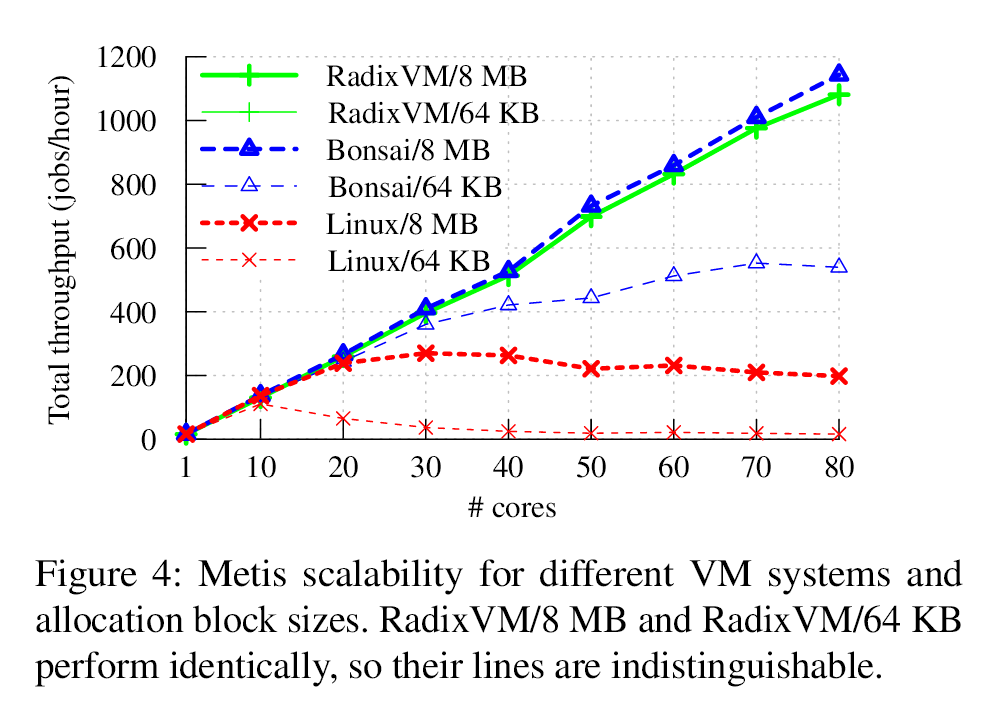
\includegraphics[width=0.4\textwidth,right]{radix}}
\end{frame}

\begin{frame}{The Scalable Commutativity Rule-Designing Scalable Software for
Multicore Processors - SOSP 13 }
    \begin{itemize}
    \item Author : Austin T.Clements : MIT PDOS
    \item Problem : 응용프로그램의 설계 문제
        \begin{itemize}
        \item Scalable한 응용프로그램
        \end{itemize}
    %\vspace{-2.5cm} 
    %\only<1>{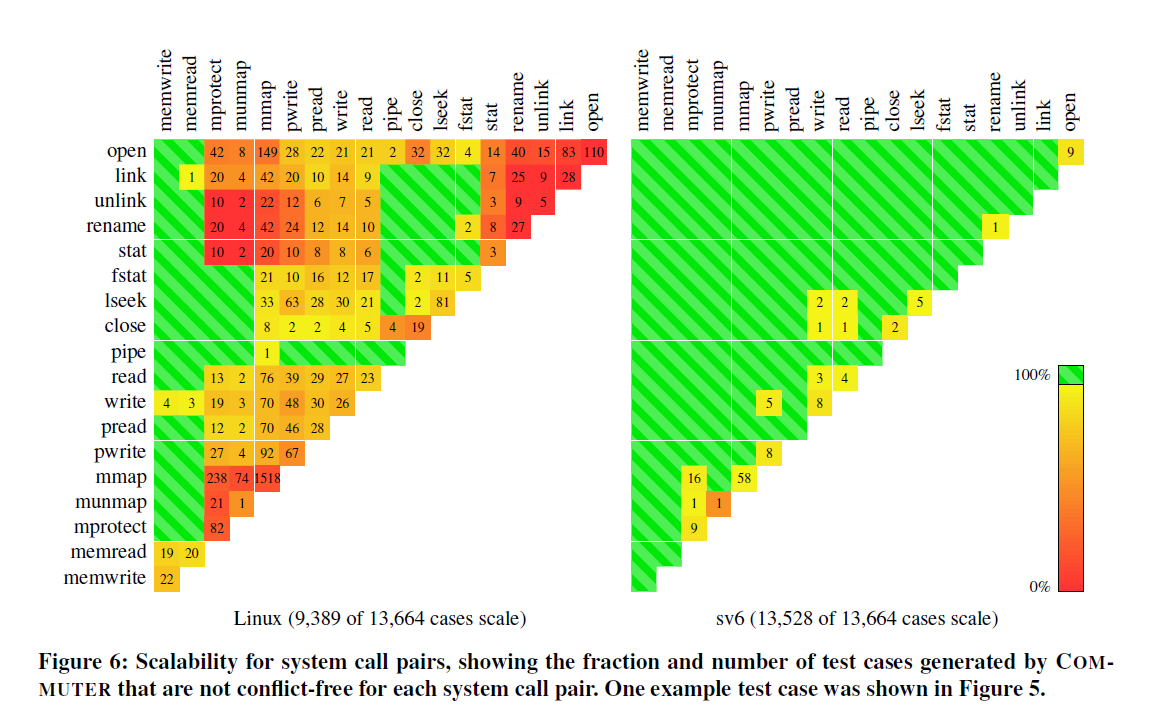
\includegraphics[width=0.5\textwidth,right]{comute}}
    \end{itemize}
\end{frame}

\begin{frame}{Scalable data structure}
\pgfdeclareimage[width=\paperwidth]{background_2_2}{.//slides/background_2_2}
\begin{textblock}{1}(0,0)
\pgfuseimage<+->{background_2_2}
\end{textblock}
\end{frame}


\begin{frame}{Scalable data structure - stack}
\pgfdeclareimage[width=\paperwidth]{background_4}{.//slides/background_4}
\begin{textblock}{1}(0,0)
\pgfuseimage<+->{background_4}
\end{textblock}
\end{frame}


\begin{frame}{Scalable data structure - list}
\pgfdeclareimage[width=\paperwidth]{background_3}{.//slides/background_3}
\begin{textblock}{1}(0,0)
\pgfuseimage<+->{background_3}
\end{textblock}
\end{frame}


\begin{frame}{More than you ever wanted to know about synchronization: synchrobench, measuring
the impact of the synchronization on concurrent algorithms - PPoPP 2015}
    \begin{itemize}
    \item Author : Vincent Gramoli - NICTA 
    \item 최신 알고르즘을 정리 또는 구현 후 공개소스로 공개
    \item 성능 측정
    \end{itemize}
\end{frame}

\begin{frame}{More than you ever wanted to know about synchronization}
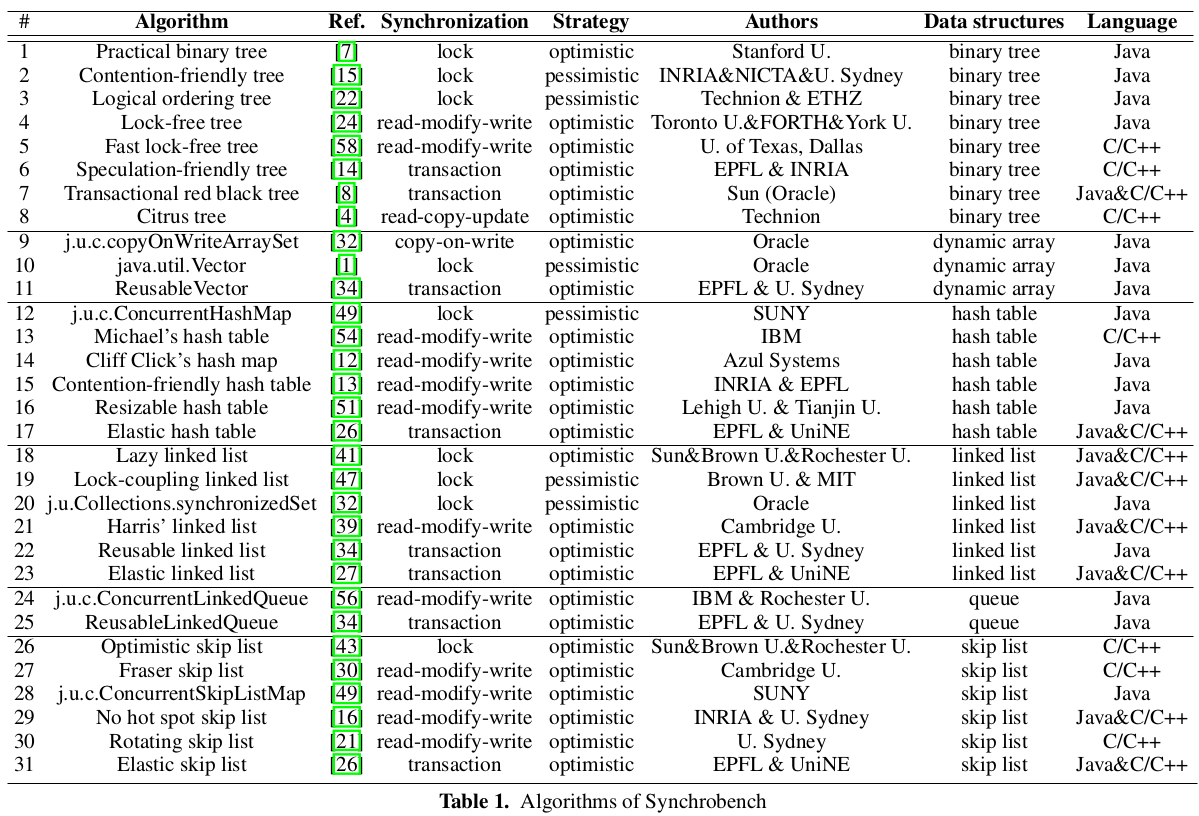
\includegraphics[width=\textwidth,height=0.8\textheight,
keepaspectratio]{algorithm}
\end{frame}


\begin{frame}{Scalable lock}
\pgfdeclareimage[width=\paperwidth]{background_2_3}{.//slides/background_2_3}
\begin{textblock}{1}(0,0)
\pgfuseimage<+->{background_2_3}
\end{textblock}
\end{frame}

\begin{frame}{exclusive lock - spin lock}
    \begin{itemize}
    \item test and set
    \item ticket lock
    \item Anderson Queue Lock
    \item MCS
    \item 등등등
    \end{itemize}
\end{frame}

\begin{frame}{concurrent reads - read-mostly data structure}
    \begin{itemize}
    \item read-write lock
    \item RCU
    \item RLU (SOSP '15)
    \end{itemize}
\end{frame}


\begin{frame}{AIM7 Scalability - Linux 4.5.0}
\pgfdeclareimage[width=\paperwidth]{background_1}{.//slides/background_1}
\begin{textblock}{1}(0,0)
\pgfuseimage<+->{background_1}
\end{textblock}
\end{frame}


\begin{frame}{Concurrent updates}
\pgfdeclareimage[width=\paperwidth]{update_lock}{.//slides/update_lock}
\begin{textblock}{1}(0,0)
\pgfuseimage<+->{update_lock}
\end{textblock}
\end{frame}

\begin{frame}{log-based concurrent updates}
    \begin{itemize}
    \item FC(Flat Combining)
    \item Oplog
    \item LDU
    \end{itemize}
\end{frame}

\begin{frame}{Flat Combining}
    \begin{itemize}
    \item Flat Combining and the Synchronization-Parallelism Tradeoff
    \item SPAA 2010
    \end{itemize}
\end{frame}


\begin{frame}{Flat Combining}
\pgfdeclareimage[width=\paperwidth]{background_5}{.//slides/background_5}
\begin{textblock}{1}(0,0)
\pgfuseimage<+->{background_5}
\end{textblock}
\end{frame}


\begin{frame}{Optimizing Communication Bottlenecks in Multiprocessor Operating
System kernels - MIT Doctor thesis 2014 }
    \begin{itemize}
    \item Author : Silas Boyd-Wickizer - MIT PODS
    \item Problem : Update-heavy datastructure
        \begin{itemize}
        \item Update-heavy한 상황
        \end{itemize}
    \item Solution : OpLog
        \begin{itemize}
        \item 새로운 lock 툴 제공
        \item synchronized clocks(RDTSC and RDTSCP)을 이용
        \item per-cpu로 데이터 저장 후 처음 read 발생 시 처리 
        \item path name looup, VM reverse mapping, and the state() system call
        \end{itemize}
    \end{itemize}
\end{frame}

\begin{frame}{Optimizing Communication Bottlenecks in Multiprocessor Operating
System kernels - MIT Doctor thesis 2014 }
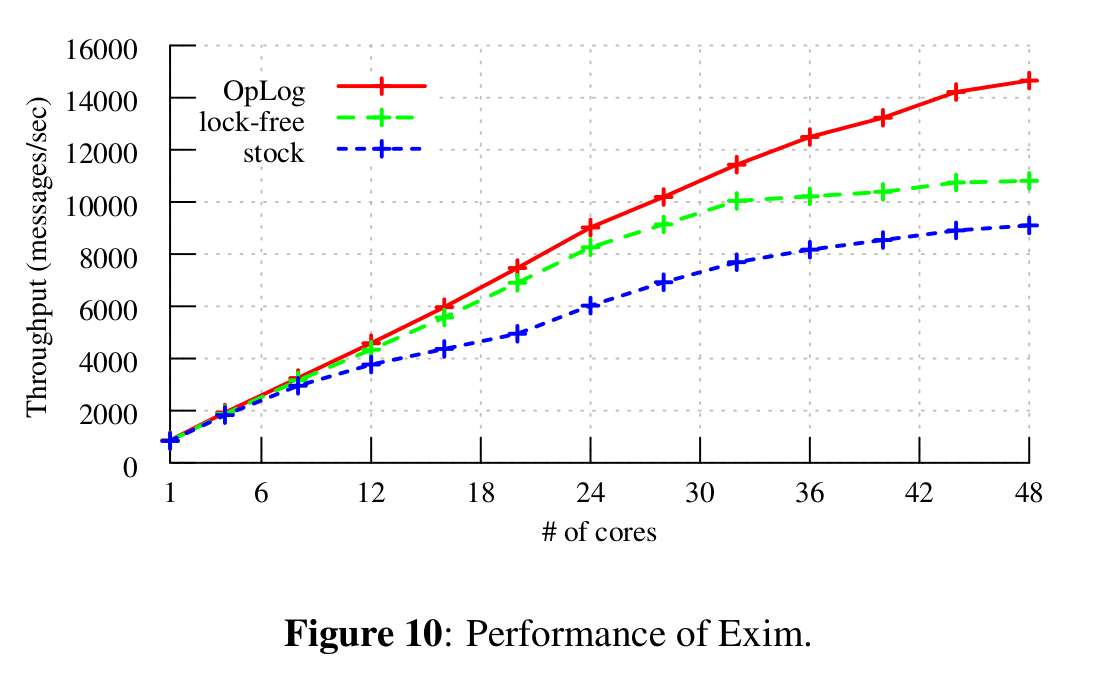
\includegraphics[width=\textwidth,height=0.7\textheight,
keepaspectratio]{oplog}
\end{frame}


\begin{frame}{Concurrent updates - solution}
\pgfdeclareimage[width=\paperwidth]{solution_3}{.//slides/solution_3}
\begin{textblock}{1}(0,0)
\pgfuseimage<+->{solution_3}
\end{textblock}
\end{frame}


\begin{frame}{Concurrent updates - solution}
\pgfdeclareimage[width=\paperwidth]{solution_5}{.//slides/solution_5}
\begin{textblock}{1}(0,0)
\pgfuseimage<+->{solution_5}
\end{textblock}
\end{frame}




\begin{frame}{Synchronized timestamp counter}
\pgfdeclareimage[width=\paperwidth]{ldu_log}{.//slides/ldu_log}
\begin{textblock}{1}(0,0)
\pgfuseimage<+->{ldu_log}
\end{textblock}
\end{frame}



\begin{frame}{removing}
\pgfdeclareimage[width=\paperwidth]{ldu_log 2}{.//slides/ldu_log_2}
\begin{textblock}{1}(0,0)
\pgfuseimage<+->{ldu_log 2}
\end{textblock}
\end{frame}


\begin{frame}{LDU}
\pgfdeclareimage[width=\paperwidth]{ldu}{.//slides/ldu}
\begin{textblock}{1}(0,0)
\pgfuseimage<+->{ldu}
\end{textblock}
\end{frame}



\begin{frame}{AIM7}

\includegraphics[width=\textwidth,height=0.8\textheight,
keepaspectratio]{aim7}
\end{frame}


\begin{frame}{exim}
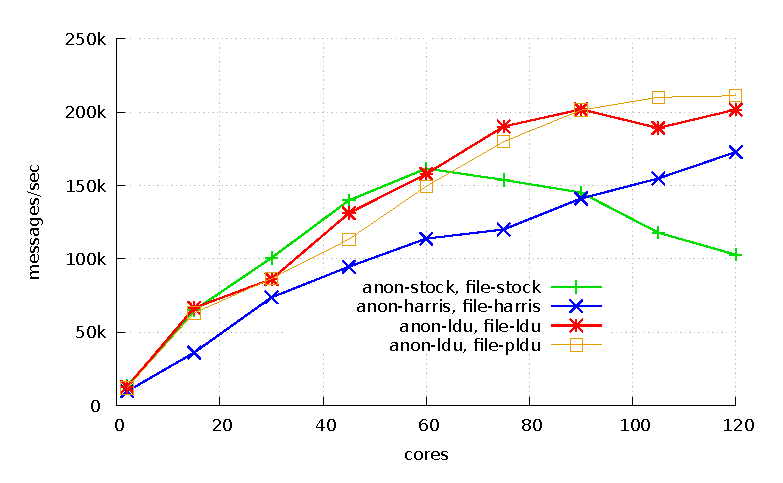
\includegraphics[width=\textwidth,height=0.8\textheight,
keepaspectratio]{exim}
\end{frame}


\begin{frame}{lmbench}
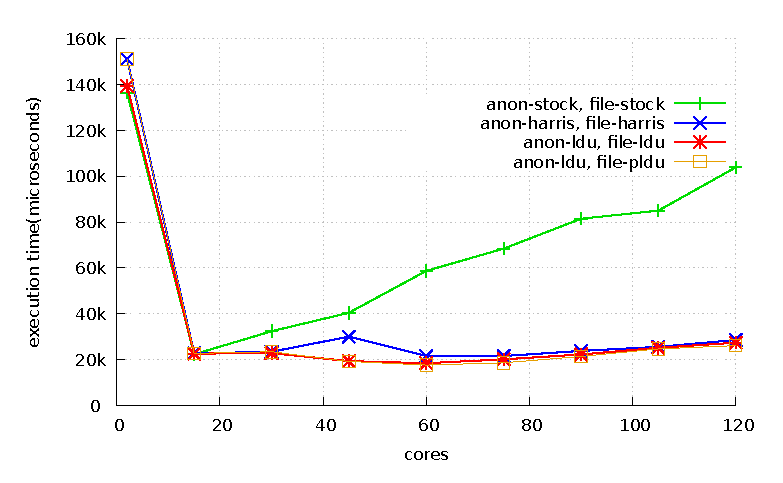
\includegraphics[width=\textwidth,height=0.8\textheight,
keepaspectratio]{lmbench}
\end{frame}



\begin{frame}{Summary}
	\begin{itemize}
	\item Background of research 
	\item LDU method and Evaluation
	\item Future plans and Summary
	\item \text{https://github.com/KMU-embedded/scalablelinux}
	\end{itemize}
\end{frame}


\end{document}
